\section{Evaluation}
\label{sec:evaluation}

Evaluation is organised around three questions: is the software mature
(Sections~\ref{sec:testing}--\ref{sec:cross-validation}); is it reliable and what
does validation buy the user (Sections~\ref{sec:fault-injection} and
\ref{sec:validation-study}--\ref{sec:live-benchmark}); and does integration offer
a measurable advantage over an unintegrated manual workflow
(Sections~\ref{sec:performance} and \ref{sec:workflow-comparison}). Throughout,
each reported figure states the script that produced it; every script referenced
is included in the software repository (Section~\ref{sec:availability}) and is
runnable independently of this manuscript. Every number in the validation study
(Sections~\ref{sec:validation-study}--\ref{sec:case-study}) is generated from the
results files by a single script rather than typed.

\subsection{Software testing}
\label{sec:testing}

The offline test suite comprises 470 tests requiring no network access,
organised one module per source area, exercised against a scripted HTTP
transport (Section~\ref{sec:architecture}) so that every failure-path
scenario in Section~\ref{sec:fault-injection} is deterministic rather than
dependent on a real service failing at a convenient moment. A further 32
tests cross-validate core calculations against Biopython
(Section~\ref{sec:cross-validation}) and are included automatically when
Biopython is installed, for a total of 502 tests. \todoinline{Confirm and
insert the authoritative \texttt{pytest --cov} statement-coverage
percentage here (the offline, stdlib-trace-based sandbox measurement used
during development was 89.4\% overall, 89.8\% restricted to the
\texttt{core}, \texttt{structures}, and \texttt{services} packages,
excluding four Tkinter view modules that cannot execute on a headless
runner; the authoritative figure should come from \texttt{pytest-cov} in
the installed environment listed in Table~\ref{tab:environment}).} A
continuous-integration matrix (GitHub Actions) runs the suite across
Python 3.10--3.13 on Linux, macOS, and Windows; a dedicated job installs the
package with no optional extras and fails the build if any third-party
import is reachable from the \texttt{core} package, verifying the
dependency-direction claim of Section~\ref{sec:architecture} mechanically
rather than by inspection alone; a further dedicated job installs Biopython
and fails the build if the cross-validation module is skipped, so that
comparison against an independent implementation runs automatically before
every release rather than being an occasional manual check.

Writing this suite found five genuine defects in carried-forward code that had
previously appeared to function correctly, and the validation study of
Section~\ref{sec:validation-study} found a sixth, in messaging, summarised in
Table~\ref{tab:defects}. Each produced plausible-looking output rather than an
explicit error, which is offered as context for why none had been noticed
previously and as the direct justification for the scale of testing reported in
this section: a defect that fails loudly is found by using the software; a defect
that fails plausibly is found only by testing against an independent expectation.

\begin{table}[htbp]
\centering
\small
\caption{Defects identified during development of \bsi\ 2.0 by systematic
testing against independent expectations, rather than by manual use of the
software. Full descriptions and the specific test that isolates each are in
the project changelog (Section~\ref{sec:availability}).}
\label{tab:defects}
\begin{tabular}{@{}p{3.6cm}p{8.4cm}@{}}
\toprule
\textbf{Defect} & \textbf{Effect} \\
\midrule
Ambiguity-code deletion before translation &
Stripping an unresolved base (\texttt{N}) prior to codon splitting shifted
the reading frame of every downstream codon, producing a plausible but
incorrect peptide with no indication of error. \\[3pt]
Silent deletion of invalid input characters &
A stray symbol (for example \texttt{@}) copied incidentally into a pasted
sequence was removed rather than reported, masking genuine input errors. \\[3pt]
Short-input alphabet misclassification &
Nucleotide/protein alphabet detection on inputs under four residues could
confidently misclassify, since every single-letter amino-acid code is also
a valid nucleotide ambiguity code. \\[3pt]
FASTA-header accession mis-parsing &
An accession embedded in a standard header
(\texttt{sp\textbar P24941\textbar CDK2\_HUMAN}) was read from the wrong
pipe-delimited field, silently defeating the accession cross-check of
Section~\ref{sec:validation}. \\[3pt]
Stale AlphaFold model-version assumption &
Constructing the model file URL from an assumed version number, rather than
querying the prediction API, caused every AlphaFold DB retrieval to fail
once the database was republished under a later version, indistinguishable
from a genuine coverage gap without querying the authoritative source
(quantified in Section~\ref{sec:live-benchmark}). \\[3pt]
Misleading message for partial structures &
A confirmed fragment of the queried protein (identity near 100\%, accession
confirmed, low coverage) was reported as M1 with the warning that it ``does not
correspond to the requested protein'', which is false for it. Found by the
validation study (Section~\ref{sec:adversarial}); corrected with the
partial-structure qualifier (Section~\ref{sec:m0m4}). \\
\bottomrule
\end{tabular}
\end{table}

\subsection{Cross-validation against an established implementation}
\label{sec:cross-validation}

Because \bsi\ reimplements common sequence and protein calculations rather
than depending on an existing library (Section~\ref{sec:package-architecture}),
its core computations are cross-validated against Biopython
\citep{cock2009biopython} wherever a directly comparable Biopython function
exists: reverse complementation, GC content, translation under multiple
genetic-code tables, molecular weight, GRAVY, and aromaticity are asserted
to agree with Biopython to within floating-point tolerance across a fixed
set of test sequences. Two measures are checked against Biopython under an
explicitly wider, literature-justified tolerance rather than exact
agreement, with the reason for the difference stated in the test itself
rather than left implicit: isoelectric point, which is checked within
0.5\,pH units, reflecting the documented disagreement between published pKa
scales \citep{kozlowski2016ipc}, and independently checked for internal
self-consistency (net charge equal to zero at the reported isoelectric
point) regardless of agreement with any external tool; and nearest-neighbour
melting temperature, checked within 10\textdegree{}C, reflecting that
Biopython's default salt-correction model and strand concentration differ
from those used here, with the conditions in force always reported
alongside the computed value (Section~\ref{sec:core-calculations}).
Deliberate differences in ambiguity-code handling -- \bsi\ retains an
unresolved base's codon position and reports it as an unspecified residue,
for the reason given in Section~\ref{sec:core-calculations} -- are likewise
asserted as documented, expected divergence rather than treated as failures.

\subsection{Fault-injection testing}
\label{sec:fault-injection}

The retry and failure-handling behaviour of Section~\ref{sec:fault-tolerance-methods}
is evaluated with a deterministic, network-independent harness: a scripted
transport (Section~\ref{sec:architecture}) replays a defined HTTP response
sequence for every request, so the same result is obtained on every machine
and in every continuous-integration run without contacting any external
service or depending on one failing at a convenient moment. Thirteen
scenarios were evaluated, with 100 repeats each (1{,}300 simulated requests
in total): a clean successful response; one, two, or persistent HTTP 504
responses; HTTP 500, 502, or 503; HTTP 429 accompanied by a
\texttt{Retry-After} header; HTTP 404 or 403, neither of which should be
retried; a read timeout; a connection error; and an HTTP 200 response whose
body is an HTML error page rather than the expected content
(Section~\ref{sec:fault-tolerance-methods}).
Results are summarised in Figure~\ref{fig:fault-injection}.

\begin{figure}[htbp]
\centering
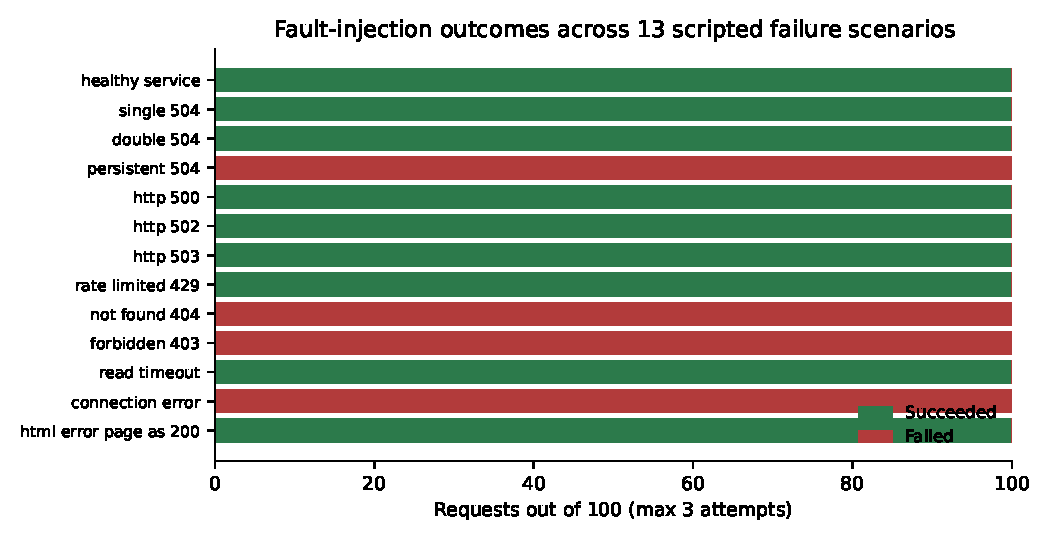
\includegraphics[width=0.92\textwidth]{figures/fault_injection}
\caption{Outcome of 1{,}300 simulated requests across 13 scripted failure
scenarios (100 repeats each). Every scenario behaved exactly as specified:
transient failures (single/double 504, 500/502/503, rate-limited 429, read
timeout, and the HTML-error-page-as-200 case) recovered in 100/100 repeats;
persistent 504 and connection-error scenarios were correctly unrecoverable
at the configured retry budget in 100/100 repeats; permanent errors (404,
403) were correctly not retried, requiring exactly one attempt in 100/100
repeats. Aggregated over the ten scenarios involving a transient or
permanent fault, 1{,}000 of 1{,}300 requests began with a failure, of which
800 (80.0\%) ultimately recovered -- the remaining 200 being the scenarios
designed to be unrecoverable.}
\label{fig:fault-injection}
\end{figure}

\subsection{Performance benchmarking}
\label{sec:performance}

Local (network-independent) computational performance was measured on the
reference machine described in Table~\ref{tab:environment}, from a fixed
random seed, and is reported separately from any measurement involving an
external service: remote response time is a property of the queried
resource, varies with time of day and geography, and is reported instead,
on its own terms, in Section~\ref{sec:live-benchmark}.

\begin{table}[htbp]
\centering
\small
\caption{Reference measurement environment for the performance figures in
this section (Section~\ref{sec:performance}); recorded automatically by the
benchmark script and included here for reproducibility.}
\label{tab:environment}
\begin{tabular}{@{}ll@{}}
\toprule
Python & CPython 3.12.3 \\
Platform & Linux x86-64 \\
Alignment cap & $4\times10^{6}$ dynamic-programming cells \\
\bottomrule
\end{tabular}
\end{table}

Single-sequence analysis completes in 0.47\,ms for a 300\,nt nucleotide
sequence, 4.1\,ms for 3{,}000\,nt, and 45.0\,ms for 30{,}000\,nt; protein
analysis completes in 0.45\,ms, 1.3\,ms, and 4.0\,ms for 100, 300, and
1{,}000 residues respectively. Batch throughput and its scaling with batch
size are shown in Figure~\ref{fig:performance}: per-sequence cost varies by
a factor of 1.16 from a batch of 10 to a batch of 1{,}000 sequences (1.10\,ms
to 1.27\,ms), indicating that throughput (786--912 sequences per second
across this range) is effectively linear in batch size over three orders of
magnitude, rather than degrading with larger batches. Semi-global alignment
cost (Section~\ref{sec:validation}), shown in Figure~\ref{fig:alignment},
scales with the dynamic-programming cell count as expected of the
underlying $O(mn)$ algorithm, from 0.59\,ms for a 76-residue query (the
length of ubiquitin) to 54.1\,ms for a 600-residue query. A cache read
(Section~\ref{sec:caching}) of a representative 200\,kB coordinate payload
completes in 0.21\,ms, roughly four orders of magnitude faster than a
typical remote structure-retrieval request (Section~\ref{sec:live-benchmark}).
Process start-up, from interpreter launch through import and a first
completed sequence analysis, takes 25.5\,ms.

\begin{figure}[htbp]
\centering
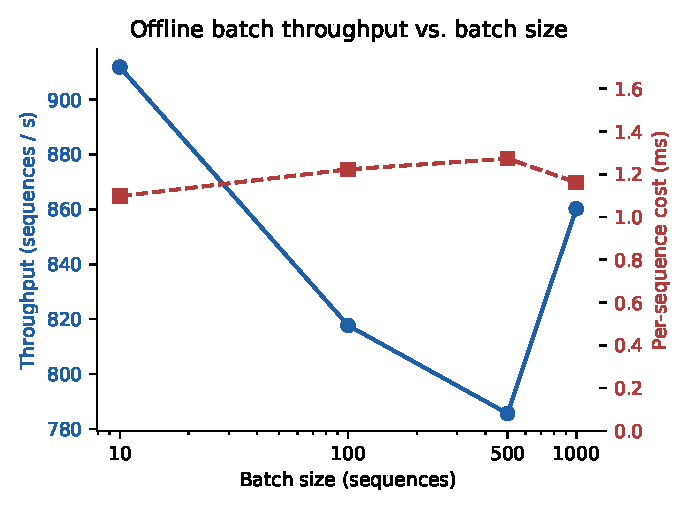
\includegraphics[width=0.62\textwidth]{figures/performance}
\caption{Offline batch-processing throughput (left axis, solid) and
per-sequence cost (right axis, dashed) as a function of batch size, on a
logarithmic horizontal axis. Per-sequence cost is stable across three orders
of magnitude in batch size.}
\label{fig:performance}
\end{figure}

\begin{figure}[htbp]
\centering
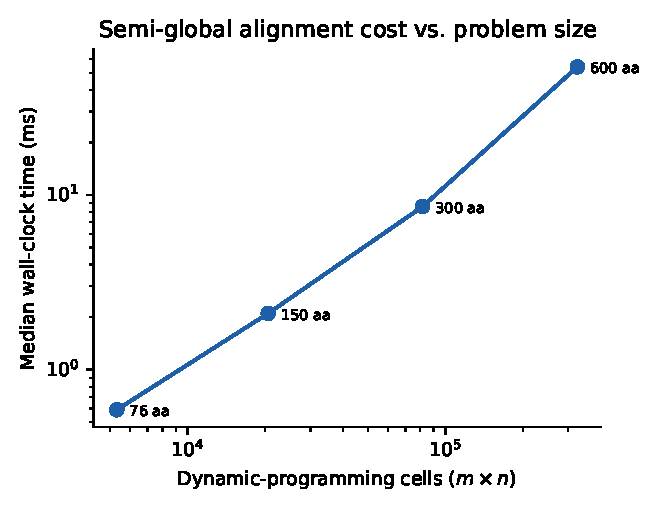
\includegraphics[width=0.55\textwidth]{figures/alignment_scaling}
\caption{Semi-global pairwise alignment (Section~\ref{sec:validation}) cost
as a function of the dynamic-programming problem size, log--log axes,
labelled by query length. Points fall close to a line of slope 1 on
log--log axes, consistent with the expected $O(mn)$ scaling.}
\label{fig:alignment}
\end{figure}

\subsection{Workflow integration}
\label{sec:workflow-comparison}

The claim that an integrated tool reduces effort relative to a manual,
multi-tool workflow is evaluated objectively rather than asserted: for five
representative tasks, a manual workflow using named, freely available web
tools is documented as an explicit, numbered list of steps (available in
full in the software repository, Section~\ref{sec:availability}), and the
number of interaction steps, distinct applications used, and manual
copy-paste data transfers between tools is counted directly from that
documented protocol -- a count that does not depend on the authors' own
software and can be independently checked or disputed against the published
step list. \bsi's equivalent step count is measured the same way against
the actual interface. This method deliberately measures interaction cost,
not human completion time or error rate, for which see the discussion of
usability evidence in Section~\ref{sec:discussion}.

\begin{table}[htbp]
\centering
\small
\caption{Interaction-cost comparison, manual multi-tool workflow versus
\bsi, across five representative tasks. T3's manual step count is the
per-sequence manual protocol (T1, 16 steps) applied across 50 sequences plus
4 batch-level steps ($50 \times 16 + 4 = 804$); \bsi's step count for T3 is
independent of the number of sequences.}
\label{tab:workflow}
\begin{tabular}{@{}p{5.4cm}rrr@{}}
\toprule
\textbf{Task} & \textbf{Manual} & \textbf{\bsi} & \textbf{Reduction} \\
\midrule
T1: single-sequence characterisation & 16 & 3 & 81.2\% \\
T2: structure retrieval with identity check & 17 & 3 & 82.4\% \\
T3: batch of 50 sequences & 804 & 3 & 99.6\% \\
T4: reproduce an earlier analysis & 6 & 3 & 50.0\% \\
T5: hand off to a collaborator & 6 & 2 & 66.7\% \\
\midrule
\textbf{Total} & \textbf{849} & \textbf{14} & \textbf{98.4\%} \\
\bottomrule
\end{tabular}
\end{table}

Table~\ref{tab:workflow} and Figure~\ref{fig:workflow} summarise the
result: across the five tasks, the documented manual workflow requires 849
steps in total against 14 for \bsi\ (98.4\% reduction), spans 16 distinct
applications against 2, and involves 17 manual copy-paste data transfers
between tools against 2. Task T2 is the task most directly relevant to this
paper's central claim: the manual protocol's steps 8--13 (extracting a
retrieved structure's chain sequence and explicitly aligning it against the
query before accepting the result) are the steps a manual workflow most
readily skips under time pressure, and skipping them is mechanistically
the failure mode measured in Section~\ref{sec:validation-study}. In
\bsi, this comparison is not an optional step a user might omit: it is
performed automatically and its result (Table~\ref{tab:m0m4}) is always
shown.

\begin{figure}[htbp]
\centering
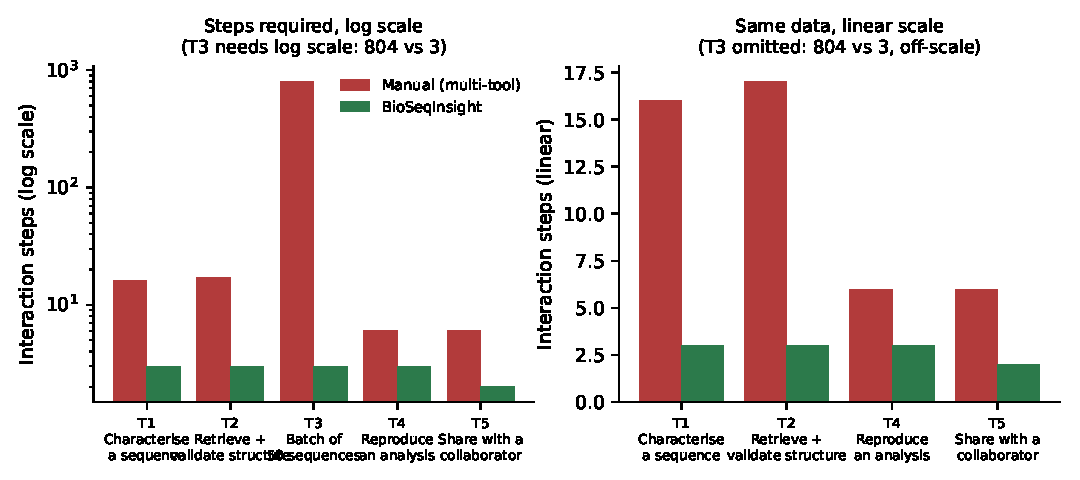
\includegraphics[width=0.92\textwidth]{figures/workflow_comparison}
\caption{Interaction steps required per task, manual multi-tool workflow
versus \bsi. Left: all five tasks, logarithmic axis (required because T3's
manual step count, 804, is two orders of magnitude larger than the
remaining tasks). Right: the same data for the four tasks whose manual step
counts do not require log scaling, linear axis.}
\label{fig:workflow}
\end{figure}

\subsection{Live service benchmark on a curated set}
\label{sec:live-benchmark}

This earlier benchmark exercises the three live services end to end (availability, latency, retrieval success) over a
curated set of 69 proteins (\texttt{benchmarks/data/benchmark\_candidates.csv}
in the software repository) selected specifically to include cases under
which naive, unvalidated structure retrieval is most likely to mislead:
near-identical paralogues (e.g.\ haemoglobin $\alpha$/$\beta$, HRas/KRas),
cross-species orthologues, a bacterial chaperonin/co-chaperonin pair
deposited together, proteins with intrinsically disordered regions,
membrane receptors deposited only as isolated domains, tandem-repeat and
precursor proteins whose deposited structures cover only a fragment of the
full-length sequence, and the human preproinsulin query that the prototype
flagged (Section~\ref{sec:case-study}). The candidate list records accession,
protein name, organism, and functional class, but deliberately \emph{not} a
pre-recorded sequence length: length, and the short/medium/long stratum
derived from it, are fetched from UniProt at benchmark run time rather than
typed in by a curator, so that a reported stratum can never silently
disagree with the sequence actually analysed.

Of the 69 candidates, 69 resolved successfully against UniProt (0
unresolved). Table~\ref{tab:livebench} and Figures~\ref{fig:livebench}--
\ref{fig:mapping} report the outcome of querying all three resources for
every resolved candidate (i.e.\ without early termination at the first
exact match, so that every resource's independent performance is visible).

\begin{table}[htbp]
\centering
\small
\caption{Live structure-resource benchmark, 69 resolved candidate proteins,
all three resources queried for every candidate. \emph{Attempted success
rate} restricts the denominator to requests actually sent (excluding
sequences ESM Atlas refuses before any request for exceeding its configured
length limit), separating genuine service unreliability from candidates a
resource cannot be asked about at all. Run captured
\texttt{2026-09-23}; software version 2.0.2; full per-protein results and
the run's internal consistency checks are included in the software
repository (Section~\ref{sec:availability}).}
\label{tab:livebench}
\begin{tabular}{@{}lrrrrr@{}}
\toprule
\textbf{Resource} & \textbf{Retrieved} & \textbf{Success} & \textbf{Attempted} & \textbf{M4 exact} & \textbf{Median} \\
 & \textbf{/ 69} & \textbf{rate} & \textbf{success rate} & \textbf{matches} & \textbf{response} \\
\midrule
RCSB PDB           & 59 & 85.5\% & 85.5\%  & 39 & 4.98\,s \\
AlphaFold DB       & 68 & 98.6\% & 98.6\%  & 68 & 0.31\,s \\
ESM Atlas          & 46 & 66.7\% & 100.0\% & 0 (predicted) & 2.04\,s \\
\bottomrule
\end{tabular}
\end{table}

\begin{figure}[htbp]
\centering
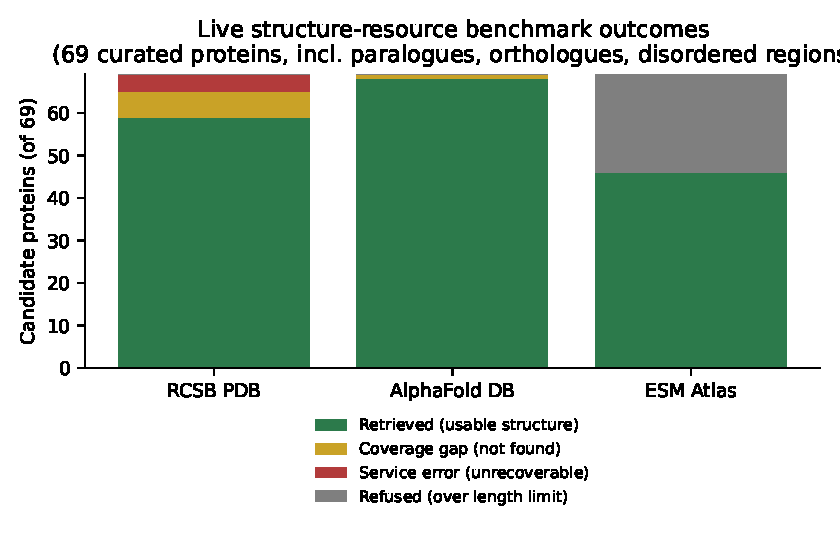
\includegraphics[width=0.72\textwidth]{figures/live_benchmark}
\caption{Outcome category per resource, live benchmark over 69 curated
proteins. ESM Atlas's 23 ``refused'' candidates are sequences exceeding its
configured length limit (400 residues), rejected before any network
request is made and reported as their own category rather than merged into
either successful retrieval or service failure.}
\label{fig:livebench}
\end{figure}

\begin{figure}[htbp]
\centering
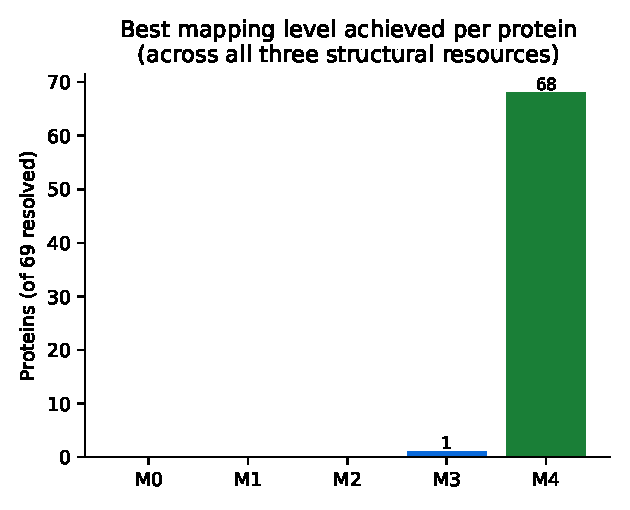
\includegraphics[width=0.5\textwidth]{figures/mapping_distribution}
\caption{Best sequence-to-structure correspondence level achieved per
protein, across all three resources (Table~\ref{tab:m0m4}). Every one of
the 69 candidates achieved at least an M3 classification; 68 (98.6\%)
achieved M4, the level supporting an unqualified statement that the
retrieved structure is the queried protein.}
\label{fig:mapping}
\end{figure}

Combining across resources, 68 of 69 candidates achieved M4 and the
remaining one M3. This figure must be read for what it is: AlphaFold DB is keyed
by UniProt accession, so its model is the queried entry by construction and
reaches M4 almost automatically; the figure is a measure of \emph{service
coverage}, not evidence that validation separates right from wrong structures,
which is the question of Section~\ref{sec:validation-study}. AlphaFold DB's
retrieval rate (98.6\%) reflects the API-discovery design of
Section~\ref{sec:retrieval}: an earlier implementation that constructed the
model file URL from an assumed, fixed model-version number achieved 0\%
retrieval on this identical candidate set once the database had been republished
under a later version -- every request returned HTTP 404, indistinguishable in
isolation from genuine absence of coverage. The comparison illustrates that a
structure-retrieval client's reliability depends on verifying assumptions against
the resource's authoritative interface, not only on the plausibility of its
request construction.


\subsection{Validation study: how often does naive retrieval return the wrong structure?}
\label{sec:validation-study}

\paragraph{Design.}
\emph{Dataset.} We sampled \N{ds-n} reviewed (Swiss-Prot) UniProt entries from
release \N{ds-release}, stratified into four equal length classes (50--150,
150--300, 300--600 and $>$600 residues) with a fixed random seed, by drawing at
random from the complete list of accessions in each class (an earlier version of
the sampler took the first results returned by the search and yielded a sample
that was entirely human; it was corrected before any result was collected). The
sample covers \N{ds-orgs} organisms, the most frequent being \emph{Homo sapiens}
at \N{ds-toporg-pct}\%. Of the \N{ds-n} proteins, \N{ds-has} have at least one PDB
entry cross-referenced in UniProt and \N{ds-no} have none; the sample is
stratified by length and category and is therefore not a representative sample of
the proteome, so rates are comparisons between policies on this set, not
estimates of prevalence.

\emph{Ground truth.} A retrieved PDB entry is judged correct for a query if the
curated databases say it contains a chain mapped to the queried accession. We
require two sources to agree: the PDBe SIFTS UniProt mapping of the entry
\citep{dana2019sifts}, and the reference-sequence identifiers RCSB
attaches to any polymer entity of the entry. Agreement gives a positive label,
joint disagreement a negative one, and a conflict is excluded as ambiguous.
Neither source is \bsi's alignment, so a correct label is not merely the
classifier restating its own output. The label is an \emph{accession-level}
claim: an identical sequence filed under a different accession is negative, and
the two sources are not independent of the cross-references the accession check
reads (Section~\ref{sec:m0m4}).

\emph{Policies.} For each query we took (i) the top RCSB sequence-search hit
with no identity filter, accepted unconditionally; (ii) the top hit of a search
carrying RCSB's own 0.9 identity cutoff, accepted unconditionally; (iii) the
\emph{same} hit as (i) accepted only if \bsi\ classifies it M4 (strict) or M3 or
better (permissive); and (iv) \bsi's own end-to-end retrieval, strict or
permissive. Policy (iii) isolates the value of the validation layer by judging
the same candidate with and without it. AlphaFold DB is accession-keyed and ESM
Atlas predicts from sequence, so neither can return a wrong accession and the
comparison is made on RCSB. The unit of analysis is the query protein. Because
\N{ds-no} proteins have no deposited structure, accepting \emph{any} structure for
them is a false association by definition; the two strata are therefore
reported separately and never blended into one headline.

\paragraph{Results.}
Table~\ref{tab:naive} and Figure~\ref{fig:outcomes} give the outcome of each
policy. Accepting the top sequence-search hit returned a structure not
catalogued under the queried accession for \N{n1-all-false} of \N{n1-all-q}
queries (\N{n1-all-far}\% of the \N{n1-all-acc} accepted hits; 95\% CI
\N{n1-all-far-lo}--\N{n1-all-far-hi}\%). For the \N{ds-has} proteins that have a
deposited structure the figure was \N{n1-has-false} of \N{n1-has-acc} returned
hits (\N{n1-has-far}\%, 95\% CI \N{n1-has-far-lo}--\N{n1-has-far-hi}\%); for the
\N{ds-no} proteins that have none, \N{n1-no-false} of \N{n1-no-acc} returned hits
(\N{n1-no-far}\%), as expected. RCSB's own identity cutoff narrows the problem
but does not remove it: \N{n2-all-false} false associations remain, \N{n2-has-false}
of \N{n2-has-acc} hits (\N{n2-has-far}\%) among proteins that have a structure.

\begin{table}[htbp]
\centering
\footnotesize\setlength{\tabcolsep}{3pt}
\caption{Outcome of five acceptance policies on \N{ds-n} proteins, judged against
curated cross-references. \emph{False} is an accession-level false association.
Sensitivity is the fraction of the \N{ds-has} proteins with a deposited structure
for which a correct structure was returned.}
\label{tab:naive}
\begin{tabular}{@{}lrrrrrrr@{}}
\toprule
 & \multicolumn{3}{c}{All \N{ds-n} queries} & \multicolumn{2}{c}{Structure exists} & \multicolumn{1}{c}{None exists} & \\
\cmidrule(lr){2-4}\cmidrule(lr){5-6}\cmidrule(lr){7-7}
\textbf{Policy} & \textbf{Accepted} & \textbf{False} & \textbf{Rate (95\% CI)} & \textbf{False/acc.} & \textbf{Sens.} & \textbf{False/acc.} & \textbf{FP/1000} \\
\midrule
Naive, top hit & \N{n1-all-acc} & \N{n1-all-false} & \N{n1-all-far}\% (\N{n1-all-far-lo}--\N{n1-all-far-hi}) & \N{n1-has-false}/\N{n1-has-acc} & \N{n1-has-sens}\% & \N{n1-no-false}/\N{n1-no-acc} & \N{n1-all-per1000} \\
Naive, RCSB 0.9 cutoff & \N{n2-all-acc} & \N{n2-all-false} & \N{n2-all-far}\% (\N{n2-all-far-lo}--\N{n2-all-far-hi}) & \N{n2-has-false}/\N{n2-has-acc} & \N{n2-has-sens}\% & \N{n2-no-false}/\N{n2-no-acc} & \N{n2-all-per1000} \\
Validated, permissive (M3+) & \N{p1-all-acc} & \N{p1-all-false} & \N{p1-all-far}\% (\N{p1-all-far-lo}--\N{p1-all-far-hi}) & \N{p1-has-false}/\N{p1-has-acc} & \N{p1-has-sens}\% & \N{p1-no-false}/\N{p1-no-acc} & \N{p1-all-per1000} \\
Validated, strict (M4) & \N{s1-all-acc} & \N{s1-all-false} & \N{s1-all-far}\% (\N{s1-all-far-lo}--\N{s1-all-far-hi}) & \N{s1-has-false}/\N{s1-has-acc} & \N{s1-has-sens}\% & \N{s1-no-false}/\N{s1-no-acc} & \N{s1-all-per1000} \\
End-to-end, strict (M4) & \N{s3-all-acc} & \N{s3-all-false} & \N{s3-all-far}\% (\N{s3-all-far-lo}--\N{s3-all-far-hi}) & \N{s3-has-false}/\N{s3-has-acc} & \N{s3-has-sens}\% & \N{s3-no-false}/\N{s3-no-acc} & \N{s3-all-per1000} \\
\bottomrule
\end{tabular}
\end{table}

\begin{figure}[htbp]
\centering
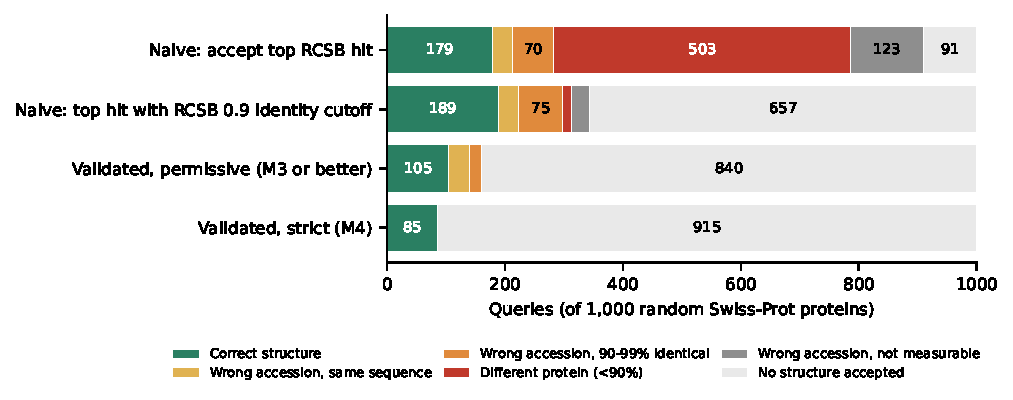
\includegraphics[width=0.95\textwidth]{figures/val_outcomes}
\caption{Outcome of four acceptance policies over all \N{ds-n} queries. False
associations are split by the measured identity of the returned hit to the query:
the same sequence under another accession, 90--99\% identical, a different
protein ($<$90\%), or not measurable (no PDB-format coordinate file exists).}
\label{fig:outcomes}
\end{figure}

\paragraph{What the false associations are.} ``False'' here means not catalogued
under the queried accession, which includes a sequence that is identical but
filed under another accession. We therefore classify each false association by
the hit's own measured identity and coverage. Of the \N{n1-all-false} naive false
associations, \N{n1-all-tier-same} are the same sequence under another accession (for
example identical histone sequences deposited under different accessions),
\N{n1-all-tier-near} are 90--99\% identical, \N{n1-all-tier-diff} are a clearly different
protein ($<$90\% identity), and \N{n1-all-tier-unm} could not be measured because the
entry has no PDB-format file. The permissive policy leaves \N{p1-all-false} false
associations, of which \N{p1-all-tier-same} are the same sequence and
\N{p1-all-tier-near} near-identical, and \emph{none} is a different protein
(\N{p1-all-tier-diff}). Among proteins that have a structure, the naive policy's
\N{n1-has-false} false associations comprise \N{n1-has-tier-same} same-sequence,
\N{n1-has-tier-near} near-identical, \N{n1-has-tier-diff} different-protein and
\N{n1-has-tier-unm} unmeasurable hits. The substantive failure of naive retrieval
is therefore real but smaller than the headline: most false associations are
proteins without any structure, for which a homologue is returned, and a minority
of those for proteins with a structure are clearly the wrong molecule.

\paragraph{The validation layer.} Accepting only M4 produced \N{s1-all-false}
false associations among \N{s1-all-acc} accepted structures (95\% CI
\N{s1-all-far-lo}--\N{s1-all-far-hi}\%), and \bsi's end-to-end strict policy
accepted \N{s3-all-acc} with \N{s3-all-false}. An exact McNemar test on the
per-query false-association outcome, naive versus strict on the same hit, has
\N{disc-n1-s1} discordant queries in one direction and none in the other
($p = \N{p-n1-s1}$), and the comparison against RCSB's cutoff policy is
\N{disc-n2-s2} versus 0 ($p = \N{p-n2-s2}$); because every discordance goes one way
these tests add little beyond the counts. Two cautions apply. The accession
component of the check and the ground truth both read curated cross-references,
so a zero here shows consistency between two views of related curated data, not
an independent audit. And unmeasurable hits cannot be accepted, so part of the
reduction is the refusal to accept what could not be checked.

\paragraph{The cost.} The strict policy returned a correct structure for
\N{s1-has-sens}\% of the proteins that have one, against \N{n1-has-sens}\% for the
naive policy (Table~\ref{tab:naive}). Figure~\ref{fig:gatecost} accounts for the
correct naive hits it did not accept: of \N{gate-total} correct hits, \N{gate-accepted}
were accepted and \N{gate-rejected} rejected, of which \N{gate-partial} were partial
structures of the right protein (accession confirmed, identity $\geq$95\%,
coverage $<$80\%), \N{gate-unmeasured} could not be validated because RCSB serves
no PDB-format file for the entry (large and recent assemblies; every case was an
HTTP 404), \N{gate-m3} were M3 (accession not confirmed) and \N{gate-other}
fell in M1 or M2. The permissive policy recovers part of this at the price of
\N{p1-all-false} false associations (none a different protein), reaching
\N{p1-has-sens}\% sensitivity. The choice between operating points is therefore a
trade-off the user can make knowingly: strict M4 for a claim that the structure
\emph{is} this protein; permissive M3+ when the same or a near-identical sequence
is acceptable.

\begin{figure}[htbp]
\centering
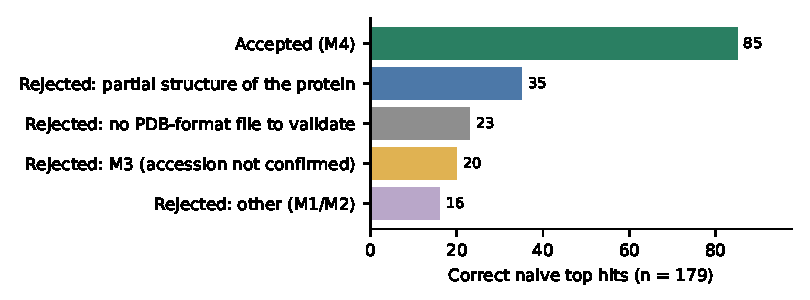
\includegraphics[width=0.78\textwidth]{figures/val_gate_cost}
\caption{What the strict (M4) policy did with the correct top hits returned by
naive retrieval. Partial structures are real structures of the queried protein
that are not full length; the partial-structure qualifier now labels them.}
\label{fig:gatecost}
\end{figure}

\subsection{Adversarial benchmark}
\label{sec:adversarial}

To test the validator on cases built to fool it, we constructed negatives from
the dataset and passed each (query, forced structure) pair directly through the
validation function, independently of any search. Table~\ref{tab:adversarial} and
Figure~\ref{fig:adversarial} report the outcome. In total \N{adv-total} cases were
built and \N{adv-scored} could be resolved and scored; the rest (\N{adv-unresolved})
had no retrievable forced structure and are excluded, which means the scored cases
are not a random subset of those built.

\begin{table}[htbp]
\centering
\small
\caption{Adversarial benchmark. Each case is a query with a forced structure
that is wrong in a specified way. Levels are the validator's output; \emph{partial}
counts results flagged as partial structures.}
\label{tab:adversarial}
\begin{tabular}{@{}p{4.4cm}rrrrrrr@{}}
\toprule
\textbf{Class (construction)} & \textbf{Scored} & \textbf{M1} & \textbf{M2} & \textbf{M3} & \textbf{M4} & \textbf{Partial} \\
\midrule
B1 wrong paralogue (same Pfam family, est.\ 40--95\% identity) & \N{adv-B1-n} & \N{adv-B1-M1} & \N{adv-B1-M2} & \N{adv-B1-M3} & \N{adv-B1-M4} & \N{adv-B1-partial} \\
B2 fragment of the right protein (SIFTS coverage $<$70\%) & \N{adv-B2-n} & \N{adv-B2-M1} & \N{adv-B2-M2} & \N{adv-B2-M3} & \N{adv-B2-M4} & \N{adv-B2-partial} \\
B4 unrelated protein (random pairing) & \N{adv-B4-n} & \N{adv-B4-M1} & \N{adv-B4-M2} & \N{adv-B4-M3} & \N{adv-B4-M4} & \N{adv-B4-partial} \\
B5 near-identical, different entry & \N{adv-B5-n} & \N{adv-B5-M1} & \N{adv-B5-M2} & \N{adv-B5-M3} & \N{adv-B5-M4} & \N{adv-B5-partial} \\
B3 other isoform (labels unverified) & \N{adv-B3-n} & \N{adv-B3-M1} & \N{adv-B3-M2} & \N{adv-B3-M3} & \N{adv-B3-M4} & \N{adv-B3-partial} \\
\bottomrule
\end{tabular}
\end{table}

\begin{figure}[htbp]
\centering
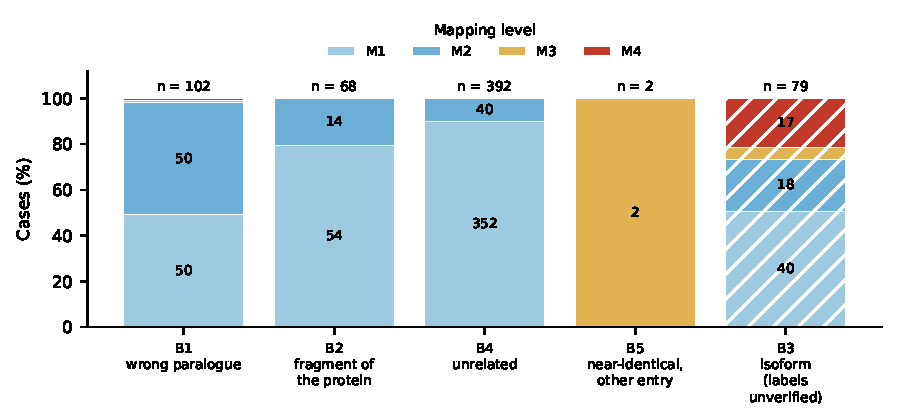
\includegraphics[width=0.78\textwidth]{figures/val_adversarial}
\caption{Mapping level reached by each adversarial class (counts shown in the
bars). Hatched: B3, whose ``wrong isoform'' label is a construction assumption
rather than ground truth.}
\label{fig:adversarial}
\end{figure}

None of the \N{adv-B4-n} unrelated pairs and none of the \N{adv-B2-n} fragments
reached M4 (or M3). Of the \N{adv-B1-n} paralogue pairs, \N{adv-B1-M1} fell to M1, \N{adv-B1-M2} to M2,
\N{adv-B1-M3} to M3 and \N{adv-B1-M4} reached M4; B5 has only \N{adv-B5-n} scored
cases and supports no conclusion. Across B1, B2, B4 and B5,
\N{adv-nonB3-M4} of \N{adv-nonB3-n} cases reached M4. A case that does reach M4
necessarily has a confirmed accession, identity $\geq$99\% and coverage $\geq$95\%,
so the forced ``paralogue'' structure in fact contains the queried protein; we
treat such a pair as a construction error (a Pfam-paired entry that is the same
protein) rather than a validator failure, but this benchmark cannot distinguish
that from an error in the cross-reference, and the case is reported, not excluded.

Two results are informative beyond the counts. First, the unrelated pairs are not
all at M1: \N{adv-B4-M2} of \N{adv-B4-n} (\N{adv-B4-M2-pct}\%) reached M2, which
Section~\ref{sec:threshold} shows is the noise floor of the alignment, not a
detection of homology. Second, B2 exposed the message defect of
Table~\ref{tab:defects}: the \N{adv-B2-accconf} fragments whose accession is
confirmed are real structures of the queried protein, yet fell to M1 or M2 with a
warning that they do not correspond to it; \N{adv-B2-partial} are now flagged as
partial structures; the others do not meet the qualifier's bounds (identity
$\geq$95\%, coverage $<$80\%), and we have not examined them individually. B3 is not interpreted as a failure rate: an isoform that
differs from the canonical sequence by a small region yields a structure that
legitimately matches the canonical query, so its ``wrong isoform'' label is not
ground truth. Restricting to the \N{adv-B3-valid-n} cases whose isoform is more than
5\% shorter than the canonical sequence (a rule fixed before the outcomes were
inspected), \N{adv-B3-valid-M4} reached M4. The adversarial set was built by a
script whose pair ordering depended on string-hash order; the file used here is
frozen and its checksum recorded, but regenerating it gives a different sample.

\subsection{Identity, coverage and accession: where the thresholds are meaningful}
\label{sec:threshold}

We used the same hits to ask which of the three measurements carries the
discrimination. Positives are the naive hits that ground truth labels correct
(\N{auc-n-npos}); negatives are the naive hits it labels wrong
(\N{auc-n-nneg}) or, separately, constructed unrelated, paralogue and
near-identical negatives (\N{auc-a-nneg}). Table~\ref{tab:auc} gives the area under
the ROC curve for identity, coverage and their product.

\begin{table}[htbp]
\centering
\small
\caption{Area under the ROC curve for separating correct hits from wrong ones.}
\label{tab:auc}
\begin{tabular}{@{}lrrrr@{}}
\toprule
\textbf{Negatives} & \textbf{n (pos/neg)} & \textbf{Identity} & \textbf{Coverage} & \textbf{Identity $\times$ coverage} \\
\midrule
Wrong naive hits & \N{auc-n-npos}/\N{auc-n-nneg} & \N{auc-n-id} & \N{auc-n-cov} & \N{auc-n-ic} \\
Constructed negatives & \N{auc-a-npos}/\N{auc-a-nneg} & \N{auc-a-id} & \N{auc-a-cov} & \N{auc-a-ic} \\
\bottomrule
\end{tabular}
\end{table}

Coverage does not add discrimination; the product scores \emph{worse} than
identity alone. The reason is that correct hits include many fragments, which
have low coverage and are the right protein: coverage measures completeness, not
whether the molecule is right. What removes the high-identity wrong hits is the
accession check. At the M4 identity and coverage thresholds (identity
$\geq$\N{th-exact-identity}\%, coverage $\geq$\N{th-exact-coverage}\%),
\N{abl-neg-ic} of \N{abl-neg} negatives would be accepted on identity and coverage
alone, and \N{abl-neg-ica} survive the accession check; of \N{abl-pos} correct
hits, \N{abl-pos-ic} pass identity and coverage and \N{abl-pos-all} pass all three.

\paragraph{The M2 threshold sits at the noise floor.} Because identity is
measured over the aligned region only, unrelated pairs can look similar by
chance. Over the \N{nf-n} unrelated pairs the median identity is \N{nf-p50-all}\%
and the 90th percentile \N{nf-p90-all}\%, but \N{nf-hilow} of these pairs reach
$\geq$50\% identity at coverage below the related threshold, a short-subject
artefact. Conditioning on coverage $\geq$\N{th-related-coverage}\%
(n = \N{nf-n-cov}) the 99th percentile identity is \N{nf-p99-cov}\%.
\N{nf-m2} of \N{nf-n} unrelated pairs (\N{nf-m2-pct}\%) satisfy the M2 criteria
(identity $\geq$\N{th-related-identity}\%, coverage $\geq$\N{th-related-coverage}\%),
\N{nf-id50} reach 50\% identity at that coverage, and \N{nf-high} reach the M3
criteria and \N{nf-exact} the M4 criteria. M2 therefore must not be read as evidence of
homology; M3 and M4 lie well above the floor. We did not retune the M2 threshold
on these data, because doing so on the evaluation set would overfit; a held-out
calibration is future work. Figure~\ref{fig:grid} shows the two joint
distributions.

\begin{figure}[htbp]
\centering
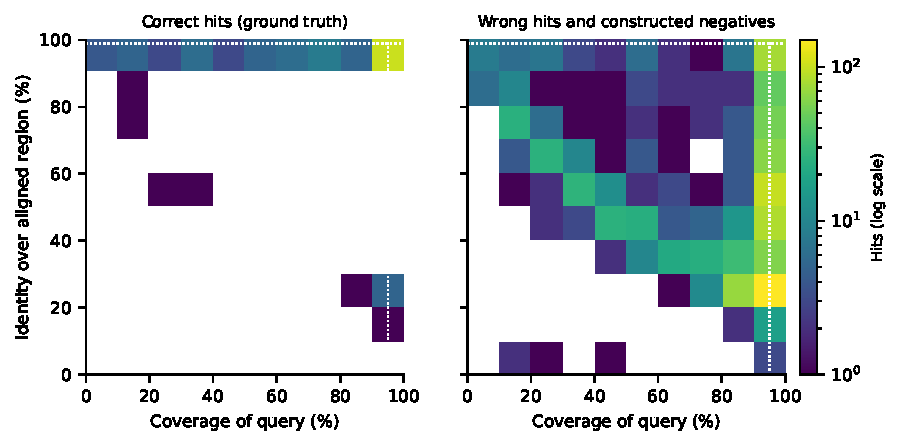
\includegraphics[width=0.9\textwidth]{figures/val_grid}
\caption{Hits by identity and coverage (10-point bins, log colour scale): correct
hits (left) concentrate at high identity and coverage, with a tail of partial
structures at high identity and low coverage; wrong hits and constructed
negatives (right) follow a diagonal in which identity rises as coverage falls.
Dotted lines mark the M4 thresholds.}
\label{fig:grid}
\end{figure}

\subsection{Re-adjudicating the 25-protein prototype benchmark}
\label{sec:case-study}

The 25 queries of the v1.0 prototype benchmark, quoted from its Table~3, were
re-run against current data (\texttt{validation/scripts/06\_case\_studies.py}). For
each, we took the top RCSB sequence-search hit, judged whether its entry
contains the queried accession (the 76-residue ubiquitin sequence, encoded
identically by four genes, counts any of them), and validated it. This reproduces
what a sequence-based retrieval returns \emph{today}; it cannot recover what v1.0
retrieved in August 2026, as the archive has changed since. Table~\ref{tab:discordance}
gives the outcome.

\begin{table}[htbp]
\centering
\small
\caption{Top RCSB sequence-search hit for the 25 prototype queries, by whether the
prototype's own report flagged an accession discordance.}
\label{tab:discordance}
\begin{tabular}{@{}lrrrrrr@{}}
\toprule
\textbf{Prototype flag} & \textbf{n} & \textbf{Entry contains accession} & \textbf{Ambiguous} & \textbf{M4} & \textbf{M3} & \textbf{$<$M3} \\
\midrule
Discordant (``mapped $\ldots$'') & \N{cs-disc-n} & \N{cs-disc-contains} & \N{cs-disc-amb} & \N{cs-disc-M4} & \N{cs-disc-M3} & \N{cs-disc-low} \\
Not flagged & \N{cs-oth-n} & \N{cs-oth-contains} & \N{cs-oth-amb} & \N{cs-oth-M4} & \N{cs-oth-M3} & \N{cs-oth-low} \\
\bottomrule
\end{tabular}
\end{table}

For \N{cs-disc-contains} of the \N{cs-disc-n} flagged queries the top hit is an
entry that contains the queried accession, and \N{cs-disc-M4} validate as M4.
The prototype's discordances therefore do not show that it retrieved wrong
structures; they show an attribution problem (the accession reported for a hit was
not always the accession of the queried chain, for example in multi-chain
complexes). Among the \N{cs-oth-n} unflagged queries, \N{cs-oth-contains} top hits
contain the accession, \N{cs-oth-amb} is ambiguous (the two curated sources
disagree), and \N{cs-oth-low} validate below M3, which shows that a hit can contain
the right accession and still be a poor structural match to the full sequence.
\textbf{This study does not support the claim that the prototype returned wrong
structures}; it motivates the larger measurement of
Section~\ref{sec:validation-study}.

